\item \points{4} {\bf Experimentation}

\begin{enumerate}[label=\alph*]
    \item Experiment with one hyperparameter that affects the performance of the model, such as the type of recurrent layer, size of hidden state, learning rate, or number of layers and submit a plot of the loss and accuracy for train and test sets.
    
    Provide a brief rationale for why you chose the parameter and what you observed in the caption for the plot.    
    
    \item \textbf{Extra Credit:} In this question we'll explore the effect of memory representation on model performance. We will focus on the $K=1$, $N=3$ case.
    
    In the previous experiments we used an LSTM model with 128 units. Consider additional memory sizes of 256, and 8. 
    
    The plots should look as follows:
    \begin{center}
        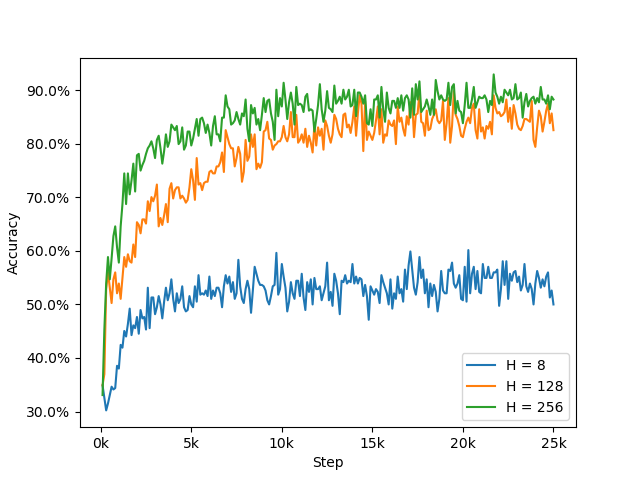
\includegraphics[width = 0.75\textwidth]{./figures/soln4ii}
    \end{center}
    
    How does increasing and decreasing the memory capacity influence performance?
        
\end{enumerate}